\documentclass[12pt,a4paper]{article}
	\pagestyle{headings}
	\title{\textbf{\Huge{descriptive.mac}\\
                       \large{A Maxima package for descriptive statistics}}}
	\author{\Large{Mario Rodr\'{\i}guez Riotorto}\\
	  \\
	  www.biomates.net\\
	  }
	\setlength{\oddsidemargin}{1cm}
	\setlength{\textwidth}{14cm}
	\setlength{\topmargin}{1.2cm}
	\setlength{\textheight}{20cm}
	\usepackage{graphicx}
	\usepackage{lscape}
	\usepackage{amsfonts}
	\usepackage{latexsym}
	\usepackage{amsmath,amsthm}
	\usepackage{color}\pagecolor{white}

	\newcommand{\normal}{\mathcal{N}}
	\newcommand{\N}{\mathbb{N}}
	\newcommand{\Z}{\mathbb{Z}}
	\newcommand{\Q}{\mathbb{Q}}
	\newcommand{\R}{\mathbb{R}}

% version: 10-06-05

\begin{document}
\maketitle
% \newpage
\tableofcontents

\section{Introduction}

The package \verb|descriptive.mac| contains a set of functions for making descriptive statistics computations and graphing. It can be downloaded, together with this document and sample data (\verb|pidigits.data|, \verb|wind.data| and \verb|biomed.data|), from the web site \emph{www.biomates.net} and is GPL licenced.

Here is a simple example on how the descriptive functions in \verb|descriptive.mac| do they work, depending on the nature of their arguments, lists or matrices,
\begin{verbatim}
(%i1) batchload("descriptive.mac")$
(%i2) /* univariate sample */
      mean([a,b,c]);
                         c + b + a
(%o2)                    ---------
                             3
(%i3) /* multivariate sample */
      matrix([a,b],[c,d],[e,f]);
                          [ a  b ]
                          [      ]
(%o3)                     [ c  d ]
                          [      ]
                          [ e  f ]
(%i4) mean(%);
                    e + c + a  f + d + b
(%o4)              [---------, ---------]
                        3          3


\end{verbatim}
Note that in multivariate samples the mean is calculated for each column.

In case of several samples with possible different sizes, the Maxima function \verb|map| can be used to get the desired results for each sample,
\begin{verbatim}
(%i5) map(mean,[[a,b,c],[d,e]]);
                      c + b + a  e + d
(%o5)                [---------, -----]
                          3        2
\end{verbatim}
In this case, two samples of sizes 3 and 2 were stored into a list.

\section{List and matrix data input}

Univariate samples must be stored in lists like
\begin{verbatim}
(%i1) s1:[3,1,4,1,5,9,2,6,5,3,5];
(%o1)       [3, 1, 4, 1, 5, 9, 2, 6, 5, 3, 5]
\end{verbatim}
and multivariate samples in matrices as in
\begin{verbatim}
(%i2) s2:matrix([13.17, 9.29],[14.71, 16.88],[18.50, 16.88],
                [10.58,  6.63],[13.33, 13.25],[13.21, 8.12]);
                      [ 13.17  9.29  ]
                      [              ]
                      [ 14.71  16.88 ]
                      [              ]
                      [ 18.5   16.88 ]
(%o2)                 [              ]
                      [ 10.58  6.63  ]
                      [              ]
                      [ 13.33  13.25 ]
                      [              ]
                      [ 13.21  8.12  ]
\end{verbatim}
In this case, the number of columns equals the random variable dimension and the number of rows is the sample size.

Data can be introduced by hand, but big samples are usually stored in plain text files. For example, file \verb|pidigits.data| contains the first 100 digits of number $\pi$:
\begin{verbatim}
      3
      1
      4
      1
      5
      9
      2
      6
      5
      3 ...
\end{verbatim}

In order to load these digits in Maxima,
\begin{verbatim}
(%i3) load("numericalio.lisp")$
(%i4) s1:read_list("pidigits.data")$
(%i5) length(s1);
(%o5)                      100
\end{verbatim}

On the other hand, file \verb|wind.data| contains daily average wind speeds at 5 meteorological stations in the Republic of Ireland\footnote{This is part of a data set taken at 12 meteorological stations. The original file is freely downloadable from the StatLib Data Repository and its analysis is discused in \cite{hasl}}. This loads the data,
\begin{verbatim}
(%i6) s2:read_matrix("wind.data")$
(%i7) length(s2);
(%o7)                      100
(%i8) s2[%]; /* last record */
(%o8)         [3.58, 6.0, 4.58, 7.62, 11.25]
\end{verbatim}

Some samples contain non numeric data. As an example, file \verb|biomed.data|\footnote{This file is part of another bigger one downloaded from the StatLib Data Repository} contains four blood measures taken from two groups of patients, \verb|A| and \verb|B|, of different ages,
\begin{verbatim}
(%i9) s3:read_matrix("biomed.data")$
(%i10) length(s3);
(%o10)                      100
(%i11) s3[1]; /* first record */
(%o11)        [A, 30, 167.0, 89.0, 25.6, 364]
\end{verbatim}
The first individual belongs to group \verb|A|, is 30 years old and his/her blood measures were 167.0, 89.0, 25.6 and 364.


One must take care when working with categorical data. In the next example, symbol \verb|a| is asigned a value in some previous moment and then a sample with categorical value \verb|a| is taken,
\begin{verbatim}
(%i12) a:1$
(%i13) matrix([a,3],[b,5]);
                          [ 1  3 ]
(%o13)                    [      ]
                          [ b  5 ]
\end{verbatim}


\section{Data manipulation}


Functions described in this section help to take some previous information from samples or to transform them. First, as this is a new Maxima session, let's read the three samples again and load package \verb|descriptive.mac|,
\begin{verbatim}
(%i1) load("numericalio.lisp")$
(%i2) s1:read_list("pidigits.data")$
(%i3) s2:read_matrix("wind.data")$
(%i4) s3:read_matrix("biomed.data")$
(%i5) batchload("descriptive.mac")$
\end{verbatim}


\begin{description}

\item[cfrec] The argument of this function must be a list of numbers, which will be then grouped in intervals and counted how many of them belong to each group. Optionally, function \verb|cfrec| admits a second argument indicating the number of classes, 10 is default,
\begin{verbatim}
(%i6) cfrec(s1,5);
(%o6) [[0, 1.8, 3.6, 5.4, 7.2, 9.0], [16, 24, 18, 17, 25]]
\end{verbatim}
The first list contains the interval limits and the second the corresponding counts: there are 16 digits inside the interval $[0, 1.8]$, that is 0's and 1's, 24 digits in $(1.8, 3.6]$, that is 2's and 3's, and so on.

\item[dfrec] Counts absolute frequencies in discrete samples, both numeric and categorical. Its unique argument is a list,
\begin{verbatim}
(%i7) dfrec(s1);
(%o7) [[0, 1, 2, 3, 4, 5, 6, 7, 8, 9],
                        [8, 8, 12, 12, 10, 8, 9, 8, 12, 13]]
(%i8) dfrec(transpose(col(s3,1))[1]);
(%o8)               [[A, B], [35, 65]]
\end{verbatim}
The first list gives the sample values and the second their absolute frequencies. Commands \verb|? col| and \verb|? transpose| should help you to understand the last input.


\item[subsample] This is a sort of variation of the Maxima \verb|submatrix| function. The first argument is the name of the data matrix, the second is a quoted logical expression and optional additional arguments are column numbers to be taken. Its behaviour is better understood with examples,
\begin{verbatim}
(%i9) subsample(s2,'(%c[1]>18));
           [ 19.38  15.37  15.12  23.09  25.25 ]
           [                                   ]
           [ 18.29  18.66  19.08  26.08  27.63 ]
(%o9)      [                                   ]
           [ 20.25  21.46  19.95  27.71  23.38 ]
           [                                   ]
           [ 18.79  18.96  14.46  26.38  21.84 ]
\end{verbatim}
These are the multivariate records in which the wind speeds in the first meteorological station were greater than 18. See that in the quoted logical expression the $i$-th component is refered to as \verb|%c[i]|. Symbol \verb|%c| is used inside function \verb|subsample|, therefore when used as a categorical variable, Maxima gets confused. In the following example, we request only the first, second and fifth components of those records with wind speeds greater or equal than 16 in station number 1 and lesser than 25 knots in station number 4,
\begin{verbatim}
(%i10) subsample(s2,'(%c[1]>=16 and %c[4]<25),1,2,5);
                  [ 19.38  15.37  25.25 ]
                  [                     ]
                  [ 17.33  14.67  19.58 ]
(%o10)            [                     ]
                  [ 16.92  13.21  21.21 ]
                  [                     ]
                  [ 17.25  18.46  23.87 ]
\end{verbatim}

Here is an example with the categorical variables of \verb|biomed.data|. We want the records corresponding to those patients in group \verb|B| who are older than 38 years,
\begin{verbatim}
(%i11) subsample(s3,'(%c[1]=B and %c[2]>38));
             [ B  39  28.0  102.3  17.1  146 ]
             [                               ]
             [ B  39  21.0  92.4   10.3  197 ]
             [                               ]
             [ B  39  23.0  111.5  10.0  133 ]
             [                               ]
             [ B  39  26.0  92.6   12.3  196 ]
(%o11)       [                               ]
             [ B  39  25.0  98.7   10.0  174 ]
             [                               ]
             [ B  39  21.0  93.2   5.9   181 ]
             [                               ]
             [ B  39  18.0  95.0   11.3  66  ]
             [                               ]
             [ B  39  39.0  88.5   7.6   168 ]
\end{verbatim}


Probably, our statistical analysis will involve only the blood measures,
\begin{verbatim}
(%i12) subsample(s3,'(%c[1]=B and %c[2]>38),3,4,5,6);
                 [ 28.0  102.3  17.1  146 ]
                 [                        ]
                 [ 21.0  92.4   10.3  197 ]
                 [                        ]
                 [ 23.0  111.5  10.0  133 ]
                 [                        ]
                 [ 26.0  92.6   12.3  196 ]
(%o12)           [                        ]
                 [ 25.0  98.7   10.0  174 ]
                 [                        ]
                 [ 21.0  93.2   5.9   181 ]
                 [                        ]
                 [ 18.0  95.0   11.3  66  ]
                 [                        ]
                 [ 39.0  88.5   7.6   168 ]
\end{verbatim}


Now, let's calculate the multivariate mean of \verb|s3|,
\begin{verbatim}
(%i13) mean(s3);
        65 B + 35 A  317          6 NA + 8145.0
(%o13) [-----------, ---, 87.178, -------------, 18.123,
            100      10                100
                                               3 NA + 19587
                                               ------------]
                                                   100
\end{verbatim}
Here, the first component is meaningless, since \verb|A| and \verb|B| are categorical, the second component is the mean age of individuals in rational form, and the fourth and last values exhibit some strange behaviour. This is because symbol \verb|NA| is used here to indicate non available data, and the two means are of course nonsense. A possible solution would be to take out from the matrix those rows with \verb|NA| symbols, although this deserves some loss of information,
\begin{verbatim}
(%i14) mean(subsample(s3,'(%c[4]#NA and %c[6]#NA),3,4,5,6));
(%o14) [79.4923076923077, 86.2032967032967,
                                                       2514
                                    16.93186813186813, ----]
                                                        13
\end{verbatim}


\end{description}


\section{Univariate descriptive statistics}

Let $(x_1, x_2, \ldots, x_n)$ be a sample of size $n$. As described in the previous section,  data can be introduced by hand or read from a file. In the following examples, \verb|s1| will store the first 100 digits of number $\pi$ and calculations will be made with them.

\begin{verbatim}
(%i1) batchload("descriptive.mac")$
(%i2) load("numericalio.lisp")$
(%i3) s1:read_list("pidigits.data")$
\end{verbatim}


\begin{description}

\item[mean] This is the sample mean, defined as
\[
\bar{x}=\frac{1}{n} \sum_{i=1}^n x_i.
\]
\begin{verbatim}
(%i4) mean(s1);
                            471
(%o4)                       ---
                            100
(%i5) numer:true$   %o4;
(%o5)                      4.71
\end{verbatim}
From now on, all results will be given in decimal notation.

\item[var, var1] There are two alternatives for the sample variance. Function \verb|var| calculates
\[
s^2=\frac{1}{n} \sum_{i=1}^n (x_i-\bar{x})^2,
\]
with division by $n$, and \verb|var1| gives
\[
s_1^2=\frac{n}{n-1}s^2.
\]
\begin{verbatim}
(%i6) var(s1);
(%o6)               8.425899999999999
(%i7) var1(s1);
(%o7)                8.5110101010101
\end{verbatim}

\item[std, std1] Function \verb|std| is the square root of $s^2$,
\[
s=\sqrt{\frac{1}{n} \sum_{i=1}^n (x_i-\bar{x})^2},
\]
and \verb|std1| is obtained from $s_1^2$
\[
s_1=\sqrt{\frac{n}{n-1}s^2}.
\]
\begin{verbatim}
(%i8) std(s1);
(%o8)               2.902740084816414
(%i9) std1(s1);
(%o9)               2.917363553109228
\end{verbatim}

\item[ncmoment, cmoment] The non central moment of order $k$ is defined as
\[
a_k=\frac{1}{n} \sum_{i=1}^n x_i^k
\]
\begin{verbatim}
(%i10) ncmoment(s1,1); /* the mean */
(%o10)                      4.71
\end{verbatim}

The central moment of order $k$ is
\[
m_k=\frac{1}{n} \sum_{i=1}^n (x_i - \bar{x})^k
\]
and calculated as
\begin{verbatim}
(%i11) cmoment(s1,2); /* the variance */
(%o11)               8.425899999999999
\end{verbatim}

\item[vc] The variation coefficient is the quotient between the sample standard deviation and the mean,
\[
\mbox{V}= \frac{s_1}{\bar{x}}.
\]
\begin{verbatim}
(%i12) vc(s1);
(%o12)               .6193977819764815
\end{verbatim}

\item[mini, maxi] These are the extreme values of the sample, the minimum
\[
x_{(1)}=\min\{x_i: 1 \leq i \leq n\},
\]
and the maximum
\[
x_{(n)}=\max\{x_i: 1 \leq i \leq n\}.
\]
\begin{verbatim}
(%i13) [mini(s1), maxi(s1)];
(%o13)                     [0, 9]
\end{verbatim}

\item[range] The range is the difference between the extreme values, $\mbox{range}=x_{(1)}-x_{(n)}$.
\begin{verbatim}
(%i14) range(s1);
(%o14)                       9
\end{verbatim}

\item[median] Once the sample is ordered, the median is the central value,
\[
\mbox{med}= \left\{ \begin{array}{ll}
               \frac{1}{2} (x_{\frac{n}{2}} + x_{\frac{n}{2} + 1}) & \mbox{if $n$ is even} \\
               x_{\frac{n+1}{2}}                               & \mbox{if $n$ is odd}
            \end{array} \right.
\]
\begin{verbatim}
(%i15) median(s1);
(%o15)                      4.5
\end{verbatim}

\item[quantile] Although there are several definitions for the sample quantile \cite{hynd}, that based on linear interpolation is implemented in \verb|descriptive.mac|. Let $(x_{(1)}, x_{(2)}, \ldots, x_{(n)})$ be the ordered sample, then the $p$-quantile, with $p \in [0,1]$, is defined as
\[
c_p= \left\{ \begin{array}{ll}
               x_{(i)} & \mbox{if $i=p n$} \\
               (p n-i)x_{(i+1)}-(p n-i-1)x_{(i)}   & \mbox{if $i < p n <i+1$}
            \end{array} \right.
\]
\begin{verbatim}
(%i16) /* 1st and 3rd quartiles */
       [quantile(s1,1/4),quantile(s1,3/4)];
(%o16)                  [2.0, 7.25]
\end{verbatim}

\item[qrange] The interquartilic range is the difference between the third and first quartiles, $c_{3/4}-c_{1/4}$,
\begin{verbatim}
(%i17) qrange(s1);
(%o17)                      5.25
\end{verbatim}

\item[meandev, mediandev] The mean deviation and the median deviation are
\[
\mbox{MD}= \frac{1}{n} \sum_{i=1}^n |x_i-\bar{x}|
\]
and
\[
\mbox{MedD}=\mbox{med}(|x_i-\mbox{med}(x_i)|),
\]
respectively.
\begin{verbatim}
(%i18) meandev(s1);
(%o18)               2.550000000000001
(%i19) mediandev(s1);
(%o19)                      2.5
\end{verbatim}

\item[harmean, geomean] The harmonic mean is defined as
\[
\mbox{H} = \frac{n}{\sum_{i=1}^n \frac{1}{x_i}}
\]
and the geometric mean as
\[
\mbox{G} = \sqrt[n]{\prod_{i=1}^n x_i}.
\]
Since the value zero appears several times in variable \verb|s1|, \verb|harmean| will give an error message and \verb|geomean| will return zero. Therefore the following example avoids the use of \verb|s1| and defines a new variable \verb|y|.
\begin{verbatim}
(%i20) y:[5,7,2,5,9,5,6,4,9,2,4,2,5]$
(%i21) [harmean(y),geomean(y)];
(%o21)     [3.901858027632205, 4.454845412337012]
\end{verbatim}

\item[kurtosis] The kurtosis coefficient is defined as
\[
\mbox{Ku}=\frac{\frac{1}{n} \sum_{i=1}^n (x_i-\bar{x})^4}{s^4} -3.
\]
\begin{verbatim}
(%i22) kurtosis(s1);

(%o22)               - 1.219988843897832
\end{verbatim}


\item[skewness] The skewness coefficient is defined as
\[
\mbox{Sk}=\frac{\frac{1}{n} \sum_{i=1}^n (x_i-\bar{x})^3}{s^3}.
\]
\begin{verbatim}
(%i23) kurtosis(s1);
(%o23)              - 1.273247946514421
\end{verbatim}

\item[pearskewness, quarskewness] The Pearson's skewness coefficient and the quartile skewness coefficient are defined as 
\[
\mbox{PSk}= \frac{3 (\bar{x}-\mbox{med}(x_i))}{s}
\]
and
\[
\mbox{QSk}= \frac{c_{3/4}-2 c_{1/2}+c_{1/4}}{c_{3/4}-c_{1/4}},
\]
respectively.
\begin{verbatim}
(%i24) pearskewness(s1);
(%o24)               .2159484029093895
(%i25) quarskewness(s1);
(%o25)               .0476190476190476
\end{verbatim}

\end{description}


\section{Multivariate descriptive statistics}


From now on, let matrix
\[
\left(
\begin{array}{cccc}
x_{11}  &  x_{12}  &  \cdots  &  x_{1d}  \\
x_{21}  &  x_{22}  &  \cdots  &  x_{2d}  \\
\vdots  &  \vdots  &          &  \vdots  \\
x_{n1}  &  x_{n2}  &  \cdots  &  x_{nd}
\end{array}
\right)
\]
be a $d$-dimensional sample of size $n$ and
\[
X_i =
\left(
\begin{array}{c}
x_{i1}  \\  x_{i2}  \\  \vdots  \\  x_{id}
\end{array}
\right) = (x_{i1}, x_{i2}, \ldots, x_{id})'
\]
the vector of observed values in the $i$-th sample unit. With such a notation, the mean vector is
\[
\bar{X} = \frac{X_1 + X_2 + \ldots +X_n}{n}.
\]


Functions introduced so far are also applicable to matrices, in which case vectors of length equal to the variable dimension will be returned. In the following examples, wind speeds measured at five meteorological stations will be used for computations,
\begin{verbatim}
(%i1) batchload("descriptive.mac")$
(%i2) load("numericalio.lisp")$
(%i3) s2:read_matrix("wind.data")$
(%i4) length(s2);  /* sample size */
(%o4)                       100
(%i5) mean(s2);  /* mean vector */
(%o5)  [9.9485, 10.1607, 10.8685, 15.7166, 14.8441]
(%i6) var(s2);  /* variances */
(%o6) [17.22190675000001, 14.98773651, 15.47572875,
                32.17651044000001, 24.42307619000001]
(%i7) maxi(s2);  /* maximum wind speed */
(%o7)      [20.25, 21.46, 20.04, 29.63, 27.63]
(%i8) kurtosis(s2);
(%o8) [- .2715445622195385, 0.119998784429451,
       - .4275233490482866, - .6405361979019522,
       - .4952382132352935]
\end{verbatim}


An important issue in multivariate statistical analysis is stochastic dependence among variables \cite{john,pena}. Measures of dependence are covariances and correlations.

\begin{description}

\item[cov, cov1] There are two alternatives for the covariance matrix, \verb|cov| computes
\[
S = \frac{1}{n} \sum_{i=1}^n X_i X_i' - \bar{X} \bar{X}'
\]
and \verb|cov1| evaluates
\[
S_1  =  \frac{n}{n-1}S 
     =    \left(
          \begin{array}{cccc}
          s_{11}  &  s_{12}  &  \cdots  &  s_{1d}  \\
          s_{21}  &  s_{22}  &  \cdots  &  s_{2d}  \\
          \vdots  &  \vdots  &          &  \vdots  \\
          s_{d1}  &  s_{d2}  &  \cdots  &  s_{dd}
          \end{array}
          \right),
\]
where $s_{ij}$ is the sample covariance between random components $X_i$ and $X_j$, and the diagonal elements $s_{ii}$ are the sample variances.

\begin{verbatim}
(%i9) fpprec:7$ /* change precision for pretty output */
(%i10) cov(s2);
       [ 17.22191  13.61811  14.37217  19.39624  15.42162 ]
       [                                                  ]
       [ 13.61811  14.98774  13.30448  15.15834  14.9711  ]
       [                                                  ]
(%o10) [ 14.37217  13.30448  15.47573  17.32544  16.18171 ]
       [                                                  ]
       [ 19.39624  15.15834  17.32544  32.17651  20.44685 ]
       [                                                  ]
       [ 15.42162  14.9711   16.18171  20.44685  24.42308 ]
(%i11) cov1(s2);
       [ 17.39587  13.75567  14.51734  19.59216  15.5774  ]
       [                                                  ]
       [ 13.75567  15.13913  13.43887  15.31145  15.12232 ]
       [                                                  ]
(%o11) [ 14.51734  13.43887  15.63205  17.50044  16.34516 ]
       [                                                  ]
       [ 19.59216  15.31145  17.50044  32.50153  20.65338 ]
       [                                                  ]
       [ 15.5774   15.12232  16.34516  20.65338  24.66977 ]
\end{verbatim}


\item[listvar] This function returns a list of global variance measures:
\begin{enumerate}
\item \emph{total variance}: $V_T=\mbox{tr}(S_1)=\sum_{i=1}^d s_{ii}$,
\item \emph{mean variance}: $V_M=\frac{\mbox{tr}(S_1)}{d}$,
\item \emph{generalized variance}: $V_G=|S_1|$,
\item \emph{generalized standard deviation}: $d_G=\sqrt{|S_1|}$,
\item \emph{efective variance} \cite{pena}: $V_E=|S_1|^\frac{1}{p}$,
\item \emph{efective standard deviation}: $d_E=|S_1|^\frac{1}{2p}$.
\end{enumerate}
\begin{verbatim}
(%i12) listvar(s2);
(%o12) [105.3383, 21.06767, 12874.35, 113.4652, 6.636591,
                                                   2.576158]
\end{verbatim}

Function \verb|listvar| has an optional logical argument: \verb|listvar(x,true)| tells Maxima that \verb|x| is the data matrix, making the same as \verb|listvar(x)|. On the other hand, \verb|listvar(x,false)| means that \verb|x| is not the data matrix, but the covariance matrix, avoiding its recalculation,
\begin{verbatim}
(%i13) listvar(%o11,false);
(%o13) [105.3383, 21.06767, 12874.35, 113.4652, 6.636591,
                                                   2.576158]
\end{verbatim}


\item[cor] The correlation matrix is defined as $R=\{r_{ij}\}_{i,j = 1, 2, \ldots, d}$, with
\[
r_{ij}=\frac{s_{ij}}{\sqrt{s_{ii} s_{jj}}}.
\]
\begin{verbatim}
(%i14) cor(s2);
       [   1.0     .8476339  .8803515  .8239624  .7519506 ]
       [                                                  ]
       [ .8476339    1.0     .8735834  .6902622  0.782502 ]
       [                                                  ]
(%o14) [ .8803515  .8735834    1.0     .7764065  .8323358 ]
       [                                                  ]
       [ .8239624  .6902622  .7764065    1.0     .7293848 ]
       [                                                  ]
       [ .7519506  0.782502  .8323358  .7293848    1.0    ]
\end{verbatim}

Function \verb|cor| has an optional logical argument: \verb|cor(x,true)| tells Maxima that \verb|x| is the data matrix, making the same as \verb|cor(x)|. On the other hand, \verb|cor(x,false)| means that \verb|x| is not the data matrix, but the covariance matrix, avoiding its recalculation,
\begin{verbatim}
(%i15) cor(%o11,false); /* this is faster */
       [   1.0     .8476339  .8803515  .8239624  .7519506 ]
       [                                                  ]
       [ .8476339    1.0     .8735834  .6902622  0.782502 ]
       [                                                  ]
(%o15) [ .8803515  .8735834    1.0     .7764065  .8323358 ]
       [                                                  ]
       [ .8239624  .6902622  .7764065    1.0     .7293848 ]
       [                                                  ]
       [ .7519506  0.782502  .8323358  .7293848    1.0    ]
\end{verbatim}

\item[listdep] This function returns a list of correlation measures:
\begin{enumerate}
\item \emph{precision matrix}: $S_1^{-1}=\{s^{ij}\}_{i,j = 1, 2, \ldots, d}$, the inverse of the covariance matrix,
\item \emph{multiple correlation vector}: $(R_1^2, R_2^2, \ldots, R_d^2)$, with $R_i^2=1-\frac{1}{s^{ii}s_{ii}}$ being an indicatior of the goodness of fit of the linear multivariate regression model on $X_i$ when the rest of variables are used as regressors.
\item \emph{partial correlation matrix}: with element $(i, j)$ being 
\[
r_{ij.\mbox{rest}}=-\frac{s^{ij}}{\sqrt{s^{ii} s^{jj}}}.
\]
\end{enumerate}
\begin{verbatim}
(%i16) z:listdep(s2)$
(%i17) fpprec:5$ /* for pretty output */
(%i18) z[1];  /* precision matrix */
       [  .38486   - .13856  - .15626  - .10239   .03118  ]
       [                                                  ]
       [ - .13856   .34107   - .15233   .03845   - .05284 ]
       [                                                  ]
(%o18) [ - .15626  - .15233   .47296   - .02482  - .10054 ]
       [                                                  ]
       [ - .10239   .03845   - .02482   .10937   - .03403 ]
       [                                                  ]
       [  .03118   - .05284  - .10054  - .03403   .14834  ]
(%i19) z[2];  /* multiple correlation vector */
(%o19)    [.85063, .80634, .86474, .71867, .72675]
(%i20) z[3];  /* partial correlation matrix */
       [  - 1.0     .38244   .36627   .49908   - .13049 ]
       [                                                ]
       [  .38244    - 1.0    .37927  - .19907   .23492  ]
       [                                                ]
(%o20) [  .36627    .37927   - 1.0    .10911    .37956  ]
       [                                                ]
       [  .49908   - .19907  .10911   - 1.0     .26719  ]
       [                                                ]
       [ - .13049   .23492   .37956   .26719    - 1.0   ]
\end{verbatim}

Function \verb|listdep| also has an optional logical argument: \verb|listdep(x,true)| tells Maxima that \verb|x| is the data matrix, making the same as \verb|listdep(x)|. On the other hand, \verb|listdep(x,false)| means that \verb|x| is not the data matrix, but the covariance matrix, avoiding its recalculation.


\end{description}



\section{Statistical graphs}

There are four types of diagrams in \verb|descriptive.mac|. Funtion \verb|dataplot| permits direct visualization of sample data, \verb|histogram| deals with the analysis of frequency patterns in continuous observations, \verb|barsplot| for categorical and discrete data frequencies and \verb|boxplot| permits to check the homocedasticity property among samples. All these functions need the external plotting program \verb|gnuplot|.

As in previous sections, the digits of $\pi$, wind speeds and blood measures will be used in the examples,
\begin{verbatim}
(%i1) batchload("descriptive.mac")$
(%i2) load("numericalio.lisp")$
(%i3) s1:read_list("pidigits.data")$
(%i4) s2:read_matrix("wind.data")$
(%i5) s3:read_matrix("biomed.data")$
\end{verbatim}

Plotting functions are now described.

\begin{description}

\item[dataplot(data, options)] The \verb|data| argument must be a numeric list or matrix, and with the \verb|options| some issues can be controlled by the user:

\begin{enumerate}
\item \verb|'outpudev|, default \verb|"x"|, indicates the output device; correct values are \verb|"x"|, \verb|"eps"| and \verb|"png"|, for the screen, postscript and png format files, respectively.
\item \verb|'maintitle|, default \verb|""|, is the main title between double quotes.
\item \verb|'axisnames|, default \verb|["x","y","z"]|, is a list with the names of axis $x$, $y$ and $z$.
\item \verb|'joined|, default \verb|false|, a logical value to select points in 2D to be joined or isolated.
\item \verb|'picturescales|, default \verb|[1.0, 1.0]|, scaling factors for the size of the plot.
\item \verb|'threedim|, default \verb|true|, tells Maxima whether to plot a three column matrix with a 3D diagram or a multivariate scatterplot. See examples bellow.
\item \verb|'axisrot|, default \verb|[60, 30]|, changes the point of view when \verb|'threedim| is set to \verb|true| and  data are stored in a three column matrix. The first number is the rotation angle of the $x$-axis, and the second number is the rotation angle of the $z$-axis, both measured in degrees.
\item \verb|'nclasses|, default \verb|10|, is the number of classes for the histograms in the diagonal of multivariate scatterplots.
\item \verb|'pointstyle|, default \verb|0|, is an integer to indicate how to display sample points.
\end{enumerate}

For example, with the following input a simple plot of the first twenty digits of $pi$ is requested and the output stored in an eps file\footnote{In this document, graphs are generated in eps format.}. The result can be seen in part \emph{a)} of Figure~\ref{fig1}.
\begin{verbatim}
(%i6) dataplot(makelist(s1[k],k,1,20),
               'outputdev="eps",'pointstyle=3)$
\end{verbatim}
Note that one dimensional data are plotted as a time series. In the next case, same more data with different settings,
\begin{verbatim}
(%i7) dataplot(makelist(s1[k],k,1,50),
             'maintitle="First pi digits",
             'axisnames=["digit order","digit value"],
             'pointstyle=1,
             'joined=true,
             'outputdev="eps")$
\end{verbatim}
The result is shown in part \emph{b)} of Figure~\ref{fig1}.


\begin{figure}
\begin{center}
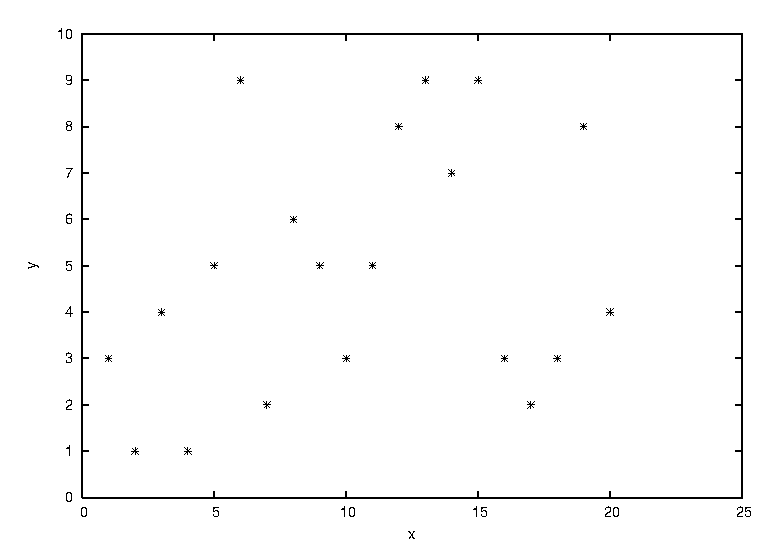
\includegraphics[scale=1.0]{dataplot1.eps} \\
\emph{a)} \\ 
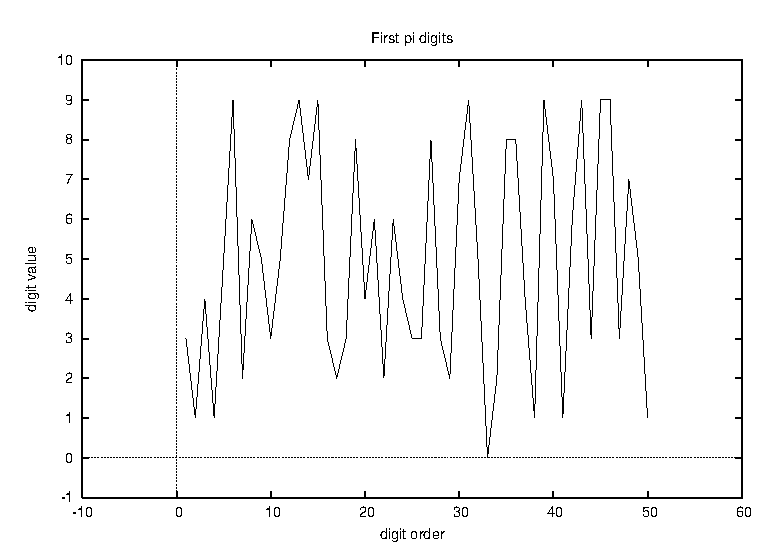
\includegraphics[scale=1.0]{dataplot2.eps} \\
\emph{b)} \\
\caption{Plotting one dimensional samples: \emph{a)} isolated points; \emph{b)} joined points.}
\label{fig1}
\end{center}
\end{figure}

Function \verb|dataplot| can be used to plot two dimensional points. The next example is a scatterplot of the pairs of wind speeds corresponding to the first and fifth meteorological stations,
\begin{verbatim}
(%i8) dataplot(submatrix(s2,2,3,4),
         'outputdev="eps", 'pointstyle=1,
         'maintitle="Pairs of wind speeds measured in knots",
         'axisnames=["Wind speed in A","Wind speed in E"])$
\end{verbatim}
The output in part \emph{a)} of Figure~\ref{fig2}

If points are stored in a two column matrix, \verb|dataplot| can plot them directly, but if they are formatted as a list of pairs, their must be transformed to a matrix as in the following example. The output is in part \emph{b)} of Figure~\ref{fig2}
\begin{verbatim}
(%i9) bs:[[64,-104], [64,-99], [61,-95], [57,-95], [55,-94],
          [55,-90], [72,-89], [80,-88], [77,-86], [80,-88], 
          [82,-91], [80,-88], [72,-89], [55,-90], [47,-89], 
          [39,-87], [33,-84], [32,-81], [35,-75], [36,-69], 
          [42,-69], [45,-68], [42,-69], [36,-69], [35,-67], 
          [35,-62], [35,-60], [39,-60], [45,-61], [51,-61], 
          [53,-65], [56,-68], [61,-70], [67,-71], [73,-70], 
          [78,-67], [80,-64], [81,-61], [78,-58], [75,-60], 
          [75,-62], [78,-62], [81,-61], [81,-56], [79,-50], 
          [75,-47], [70,-44], [62,-44], [58,-45], [53,-50], 
          [52,-52], [49,-53], [48,-52], [48,-50], [49,-48], 
          [51,-49], [52,-52], [51,-54], [51,-57], [51,-61], 
          [45,-61], [39,-60], [35,-60], [32,-57], [32,-52], 
          [32,-49], [35,-45], [39,-42], [43,-41], [48,-42], 
          [51,-43], [55,-47], [51,-43], [48,-42], [43,-41], 
          [44,-38], [47,-35], [54,-16], [56,-5], [60,-11], 
          [64,-6], [67,-12], [72,-7], [74,-14], [80,-9], 
          [80,-16], [86,-11], [87,-17], [92,-12], [93,-21], 
          [99,-16], [100,-22], [106,-19], [107,-27], [115,-25], 
          [110,-32], [94,-72], [91,-72], [88,-73], [87,-74], 
          [88,-76], [91,-76], [91,-79], [89,-81], [91,-79], 
          [91,-76], [94,-77], [94,-79], [94,-77], [91,-76], 
          [88,-76], [87,-74], [88,-73], [91,-72], [94,-72], 
          [97,-75], [98,-80], [97,-82], [94,-84], [91,-85], 
          [87,-83], [84,-80], [87,-83], [91,-85], [91,-95], 
          [92,-102], [85,-105], [69,-106], [64,-104]]$
(%i10) dataplot(apply('matrix,bs),
           'outputdev="eps",
           'maintitle="Bart", 'joined=true,
           'axisnames=["","",""],
           'picturescales=[0.5, 1.0])$
\end{verbatim}


\begin{figure}
\begin{center}
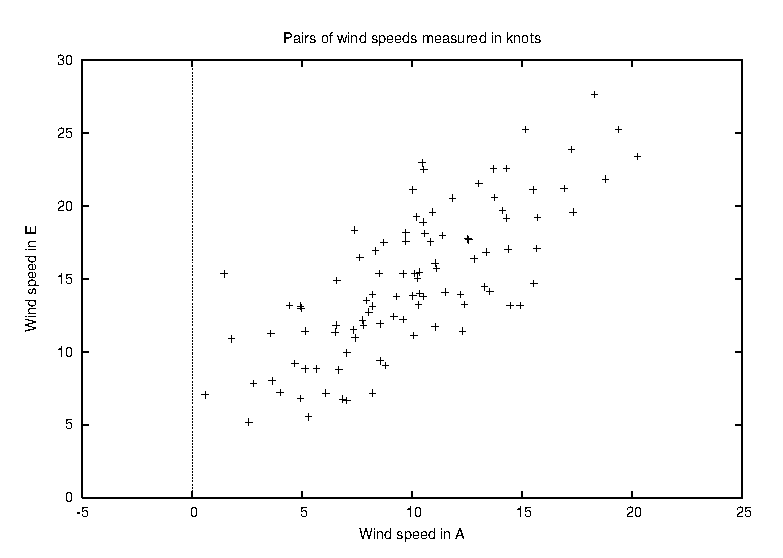
\includegraphics[scale=1.0]{dataplot3.eps} \\
\emph{a)} \\ 
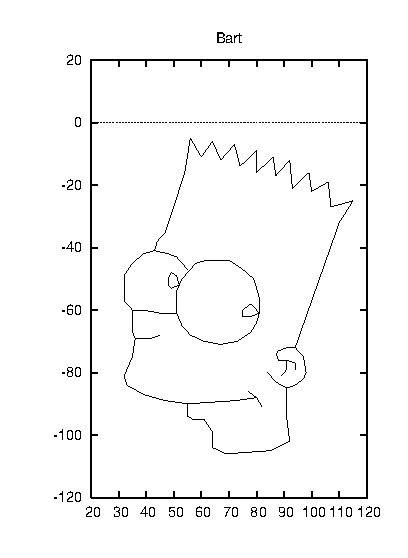
\includegraphics[scale=1.0]{dataplot4.eps} \\
\emph{b)} \\
\caption{Plotting two dimensional samples: \emph{a)} scatterplot; \emph{b)} joined points.}
\label{fig2}
\end{center}
\end{figure}

Three dimensional points can be seen as a projection on the plane. In this example, plots of wind speeds corresponding to  three meteorological stations are requested, first in a 3D plot and then in a multivariate scatterplot \cite{john}, 
\begin{verbatim}
(%i11) /* 3D plot */
       dataplot(submatrix(s2,4,5), 'pointstyle=2,
         'outputdev="eps", 'picturescales=[0.6, 0.6],
         'maintitle="Pairs of wind speeds measured in knots",
         'axisnames=["Station A","Station B","Station C"])$
(%i12) /* Multivariate scatterplot */
       dataplot(submatrix(s2,4,5),
         'outputdev="eps", 'nclasses=6, 'threedim=false)$
\end{verbatim}
Note that in the last example, the number of classes in the histograms of the diagonal is set to 6, and that option \verb|'threedim| is set to \verb|false|. Both diagrams are in Figure~\ref{fig3}.


\begin{figure}
\begin{center}
\includegraphics[scale=1.0,angle=270]{dataplot5.eps} \\
\emph{a)} \\ 
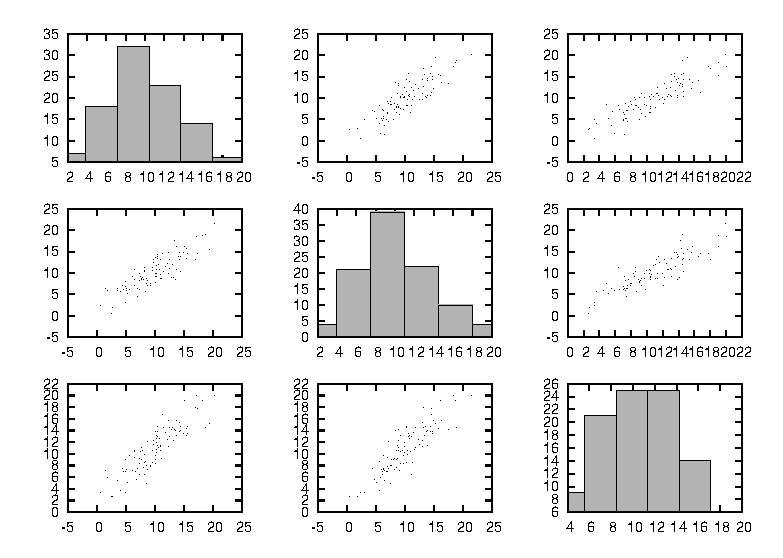
\includegraphics[scale=1.0]{dataplot6.eps} \\
\emph{b)} \\
\caption{Three dimensional samples: \emph{a)} 3D; \emph{b)} multivariate scatterplot.}
\label{fig3}
\end{center}
\end{figure}

For more than three dimensions only multivariate scatterplots are possible, as in
\begin{verbatim}
(%i13) dataplot(s2,'outputdev="eps")$
\end{verbatim}


\item[histogram(data, options)] This function plots an histogram. The \verb|data| must be stored in a list of numbers or a one column matrix. There are also some options here,

\begin{enumerate}
\item \verb|'outpudev|, default \verb|"x"|, indicates the output device; correct values are \verb|"x"|, \verb|"eps"| and \verb|"png"|, for the screen, postscript and png format files, respectively.
\item \verb|'maintitle|, default \verb|""|, is the main title between double quotes.
\item \verb|'axisnames|, default \verb|["x", "Fr."]|, is a list with the names for axis $x$ and $y$.
\item \verb|'picturescales|, default \verb|[1.0, 1.0]|, scaling factors for the size of the plot.
\item \verb|'nclasses|, default \verb|10|, is the number of classes or bars.
\item \verb|'relbarwidth|, default \verb|0.9|, a decimal number between 0 and 1 to control bar width.
\item \verb|'barcolor|, default \verb|1|, an integer to indicate bars color.
\item \verb|'colorintensity|, default \verb|1|, a decimal number between 0 and 1 to fix color intensity.
\end{enumerate}

In the next two examples, histograms are requested for the first 100 digits of number $\pi$ and for the wind speeds in the third meteorological station. Both histograms are reproduced in Figure~\ref{fig4}.
\begin{verbatim}
(%i14) histogram(s1,'maintitle="pi digits",
                 'axisnames=["","Absolute frequency"],
                 'relbarwidth=0.2,'barcolor=3,
                 'colorintensity=0.6,'outputdev="eps")$
(%i15) histogram(col(s2,3),
                 'outputdev="eps",'colorintensity=0.3)$
\end{verbatim}
Note that in the first case, \verb|s1| is a list and in the second example, \verb|col(s2,3)| is a matrix.

\begin{figure}
\begin{center}
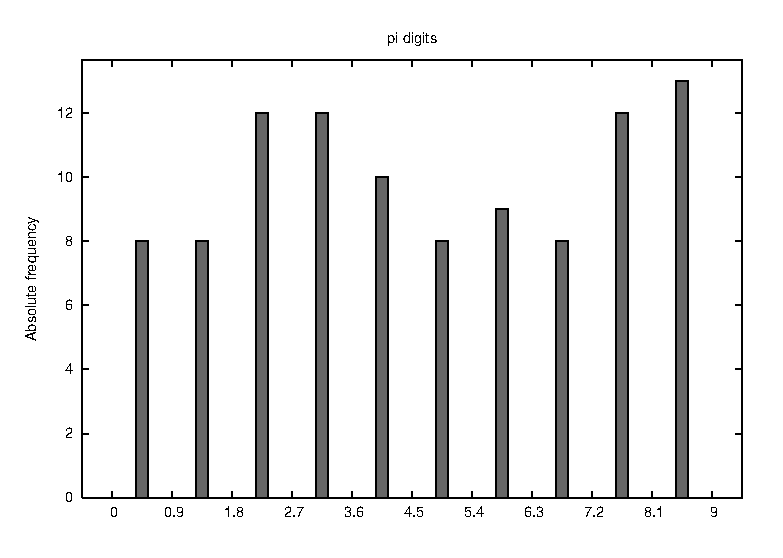
\includegraphics[scale=1.0]{histogram1.eps} \\
\emph{a)} \\ 
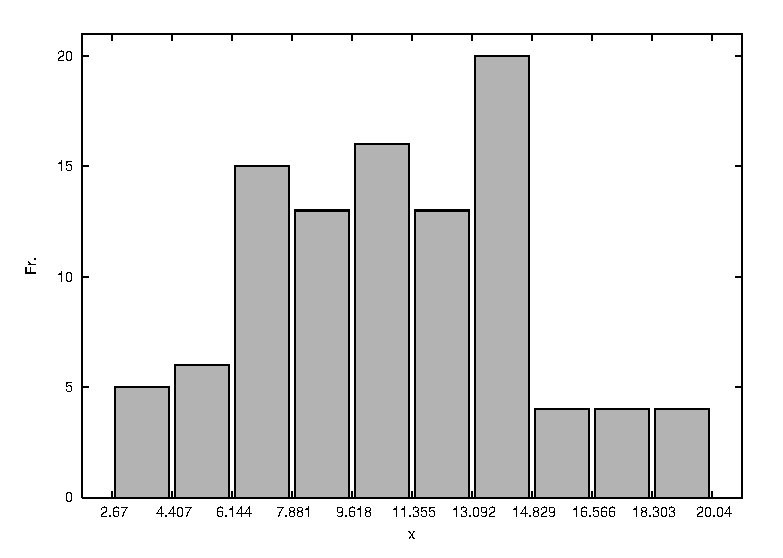
\includegraphics[scale=1.0]{histogram2.eps} \\
\emph{b)} \\
\caption{Histograms: \emph{a)} digits of $\pi$; \emph{b)} wind speeds.}
\label{fig4}
\end{center}
\end{figure}

\item[barsplot(data, options)] Similar to histograms but for discrete, numeric or categorical, statistical variables.

\begin{enumerate}
\item \verb|'outpudev|, default \verb|"x"|, indicates the output device; correct values are \verb|"x"|, \verb|"eps"| and \verb|"png"|, for the screen, postscript and png format files, respectively.
\item \verb|'maintitle|, default \verb|""|, is the main title between double quotes.
\item \verb|'axisnames|, default \verb|["x", "Fr."]|, is a list with the names for axis $x$ and $y$.
\item \verb|'picturescales|, default \verb|[1.0, 1.0]|, scaling factors for the size of the plot.
\item \verb|'relbarwidth|, default \verb|0.9|, a decimal number between 0 and 1 to control bar width.
\item \verb|'barcolor|, default \verb|1|, an integer to indicate bars color.
\item \verb|'colorintensity|, default \verb|1|, a decimal number between 0 and 1 to fix color intensity.
\end{enumerate}

First, let's obtain the barchart for groups \verb|A| and \verb|B| of patients in sample \verb|s3|,
\begin{verbatim}
(%i17) barsplot(col(s3,1),
         'outputdev="eps",
         'maintitle="Groups of patients",
         'axisnames=["Group","# of individuals"],
         'colorintensity=0.2)$
\end{verbatim}
Remember that the first column in sample \verb|s3| stores the categorical values \verb|A| and \verb|B|, also known sometimes as factors. On the other hand, the positive integer numbers in the second column are ages, in years, which is a discrete variable, so we can plot the absolute frequencies for these values,
\begin{verbatim}
(%i18) barsplot(col(s3,2),
         'outputdev="eps",
         'maintitle="Ages",
         'axisnames=["Years","# of individuals"],
         'colorintensity=0.2,
         'relbarwidth=0.6)$
\end{verbatim}

These two plots are represented in Figure~\ref{fig5}.

\begin{figure}
\begin{center}
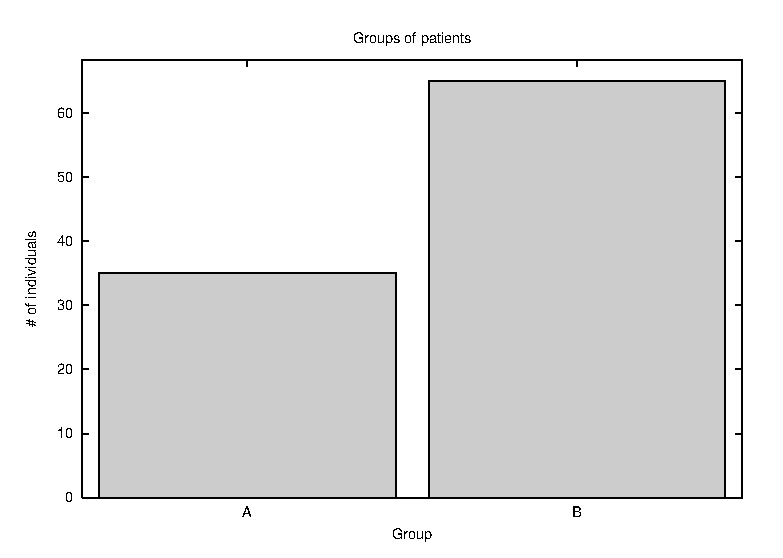
\includegraphics[scale=1.0]{barsplot1.eps} \\
\emph{a)} \\ 
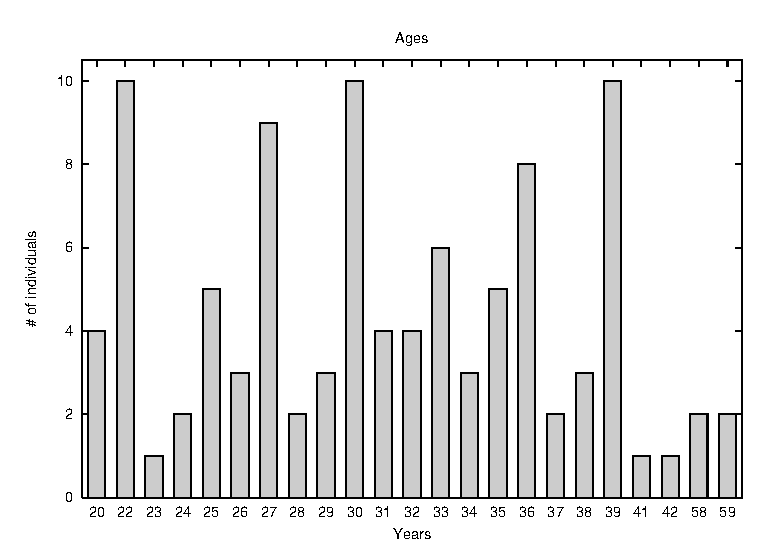
\includegraphics[scale=1.0]{barsplot2.eps} \\
\emph{b)} \\
\caption{Barcharts: \emph{a)} of categorical variable; \emph{b)} of discrete numeric variable.}
\label{fig5}
\end{center}
\end{figure}


\item[boxplot(data, options)] This function plots box diagrams. Argument \verb|data| can be a list, which is not of great interest, since these diagrams are mainly used for comparing different samples, or a matrix, so it is possible to compare two or more components of a multivariate statistical variable. But it is also allowed \verb|data| to be a list of samples with possible different sample sizes, in fact this is the only function in package \verb|descriptive.mac| that admits this type of data structure. See example bellow.

\begin{enumerate}
\item \verb|'outpudev|, default \verb|"x"|, indicates the output device; correct values are \verb|"x"|, \verb|"eps"| and \verb|"png"|, for the screen, postscript and png format files, respectively.
\item \verb|'maintitle|, default \verb|""|, is the main title between double quotes.
\item \verb|'axisnames|, default \verb|["sample", "y"]|, is a list with the names for axis $x$ and $y$.
\item \verb|'picturescales|, default \verb|[1.0, 1.0]|, scaling factors for the size of the plot.
\end{enumerate}

The outputs of these two examples are in Figure~\ref{fig6}. Remember that each box is constructed with the extremes and quartiles of the samples.
\begin{verbatim}
(%i19) boxplot(s2,'outputdev="eps",
               'maintitle="Velocidad del viento en nudos",
               'axisnames=["Estaciones",""])$
(%i20) boxplot([[6,4,6,2,4,8,6,4,6,4,3,2],
               [8,10,7,9,12,8,10],
               [16,13,17,12,11,18,13,18,14,12]],
             'outputdev="eps")$
\end{verbatim}


\begin{figure}
\begin{center}
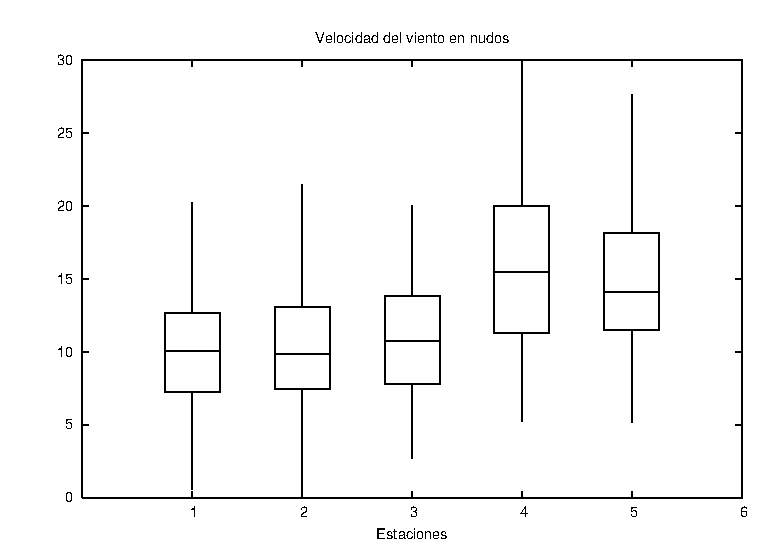
\includegraphics[scale=1.0]{boxplot1.eps} \\
\emph{a)} \\ 
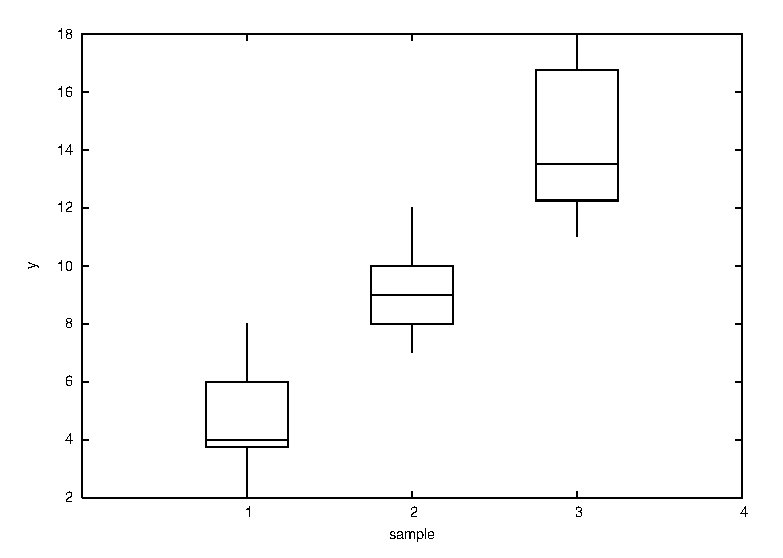
\includegraphics[scale=1.0]{boxplot2.eps} \\
\emph{b)} \\
\caption{Box plots: \emph{a)} meteorological data; \emph{b)} three samples of different size.}
\label{fig6}
\end{center}
\end{figure}


\end{description}


\bibliographystyle{plain}

\begin{thebibliography}{10}

\bibitem{hasl}
Haslett, J., Raftery, A. E. (1989) \emph{Space-time Modelling with
   Long-memory Dependence: Assessing Ireland's Wind Power Resource
   (with Discussion)}. Applied Statistics \textbf{38}, 1--50.

\bibitem{hynd}
Hyndman, R. J., Fan, Y. (1996) \emph{Sample quantiles in statistical
     packages}. American Statistician, \textbf{50}, 361--365.

\bibitem{john}
Johnson, A.J., Wichern, D.W. (1998) \emph{Applied Multivariate Statistical
      Analysis}. Prentice Hall.

\bibitem{pena}
Pe\~{n}a, D. (2002) \emph{An\'alisis de datos multivariantes}. McGraw-Hill, Madrid.

\bibitem{rios}
R\'{\i}os, S. (1985) \emph{M\'etodos estad\'isticos}. Ed. del Castillo, Madrid.




\end{thebibliography}

\end{document}

